\documentclass{beamer}
\usetheme{Montpellier}
%\usetheme{Berlin}

\usepackage{xltxtra}
\usepackage{fontspec} %指定新罗马字体
\usepackage{float}
\usepackage{listings} % 代码
\usepackage{xeCJK}  %指定中文字体
\usepackage{epigraph}
\usepackage{amsmath}
\usepackage{underscore}
\setmainfont{Times New Roman}
\setsansfont{Helvetica}
\setmonofont{Courier}
\setCJKmainfont[BoldFont={STXihei},ItalicFont={STKaiti}]{STSong}

\setbeamertemplate{headline}{
%\begin{beamercolorbox}{section in head/foot}
%   \vskip2pt \hspace{2mm} \inserttitle \vskip2pt
%\end{beamercolorbox}
\begin{beamercolorbox}{section in head/foot}
   \vskip2pt\insertnavigation{\paperwidth}\vskip2pt
\end{beamercolorbox}
\begin{beamercolorbox}[colsep=1.5pt,ht=.35ex]{upper separation line head}                   % separator
\end{beamercolorbox}
} 
%\useoutertheme{infolines}

\title[kubernetes]{一些概念简单介绍}

\author{蔚雷}

\date{\today}

\begin{document}


\frame{\titlepage}  
  
\section*{目录}   
  
\frame{\tableofcontents}  
  
%\section{介绍}  
%  
%\frame { \frametitle{这里是中文} \begin{itemize}  
%  
%\item<1-> Normal LaTeX class.  
%  
%\item<2-> this is "中文".   
%  
%\item<3-> No external programs needed.   
%  
%\end{itemize} }  

\section{ 介绍}

\begin{frame}

	\begin{itemize}
		\item kubernetes 也是master-slave架构,支持docker,rocket做为底层容器引擎,
		\item 可以随时伸缩容器集群,支持在线升级。
		\item 监控容器以达到预期目的。
	\end{itemize}
\end{frame}
\section{kubernetes master}

%\begin{frame}
%  \begin{columns}[T]
%    \begin{column}{.5\textwidth}
%     \begin{block}{Your textblock}
%	     master
%    \end{block}
%    \end{column}
%    \begin{column}{.5\textwidth}
%    \begin{block}{Your image}
%% Your image included here
%    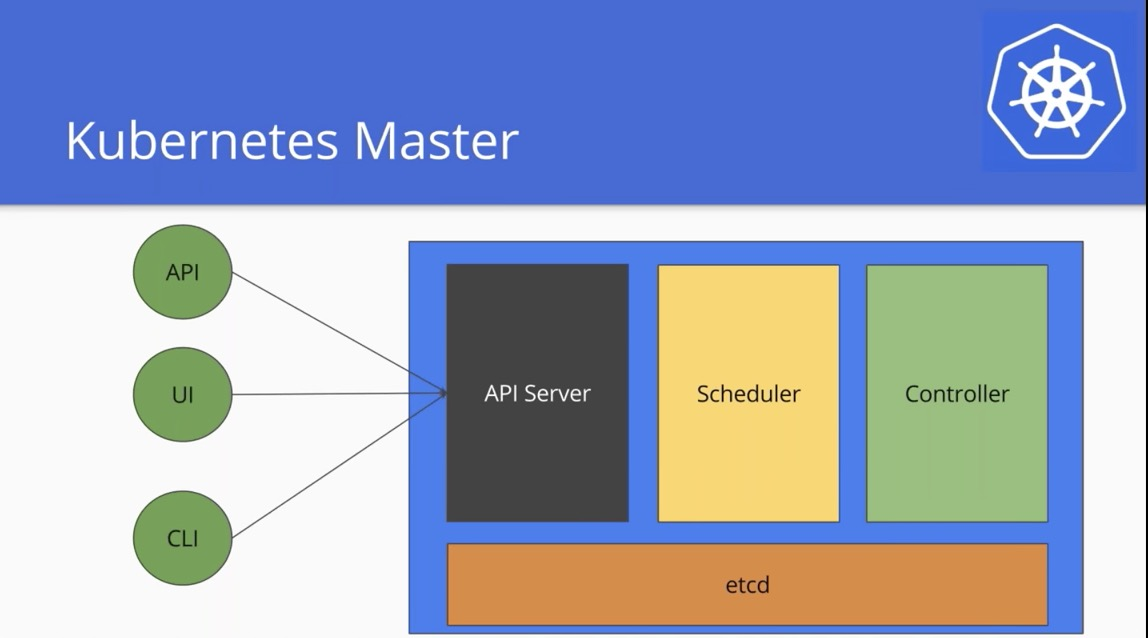
\includegraphics[width=\textwidth>]{../kubernetes-101/images/kubernetes-master.png}
%    \end{block}
%    \end{column}
%  \end{columns}
%\end{frame}
\begin{frame}[fragile]
	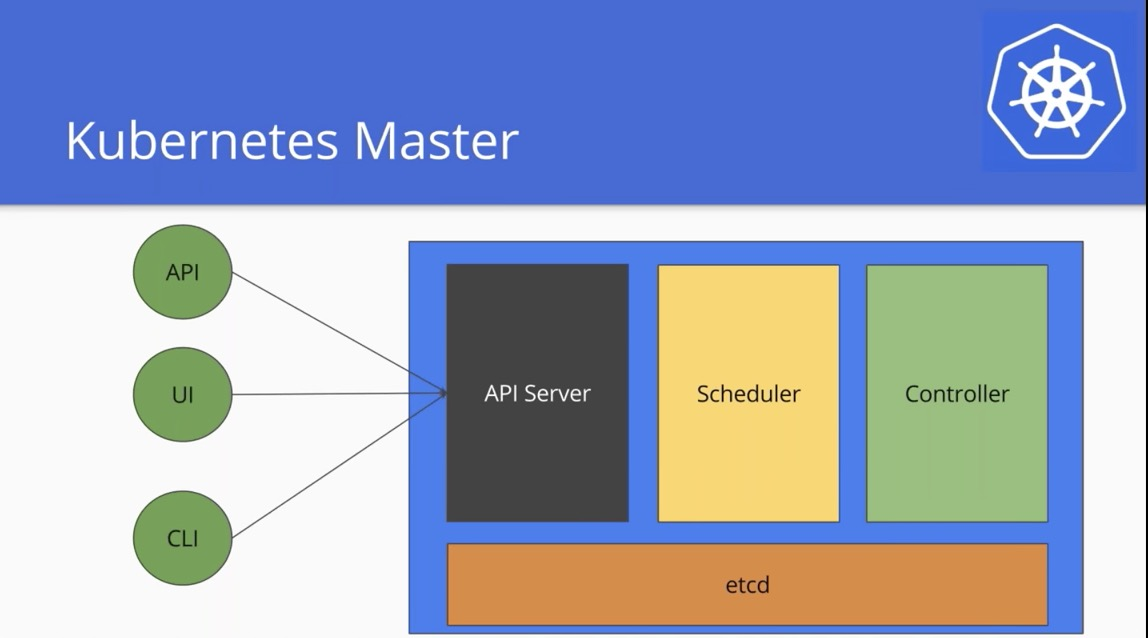
\includegraphics[width=\textwidth,scale=0.6]{../kubernetes-101/images/kubernetes-master.png}
	\begin{itemize}
		\item apiserver 管理k8s所有资源对象,与其他模块数据交互和通信的枢纽,提供用户接口,
		\item scheduler 调度pod分配到集群的那个nodes上。
		\item controller manager 监控资源变化,以达到预期目的。
	\end{itemize}

\end{frame}


\section{kubernetes node}

\frame{
	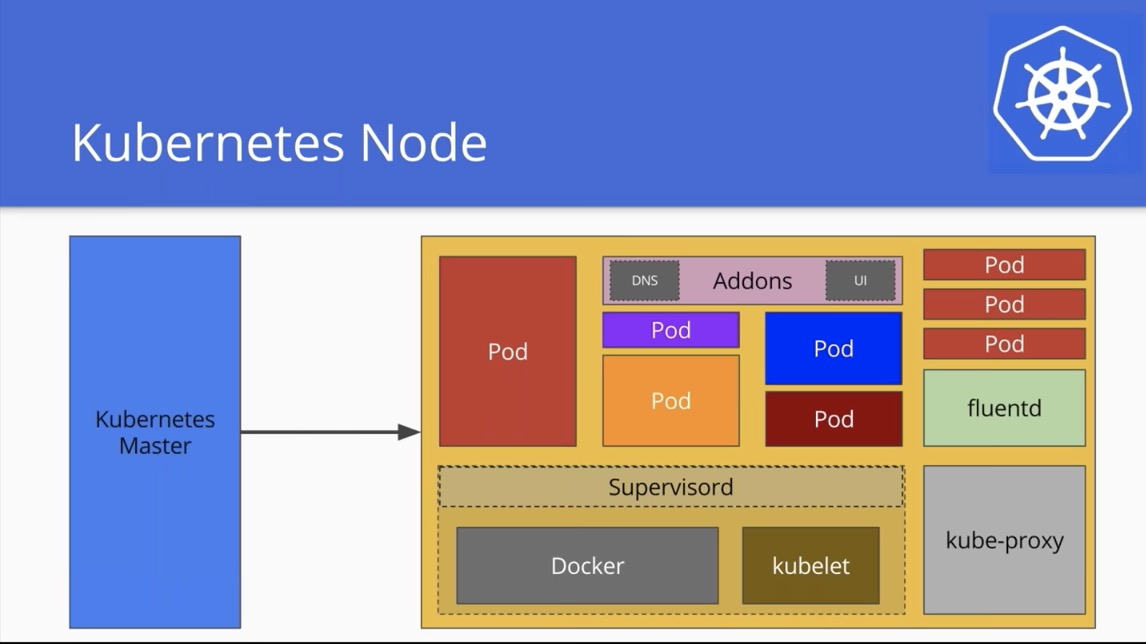
\includegraphics[width=\textwidth,scale=0.6]{../kubernetes-101/images/kubernetes-node.png}
	\begin{itemize}
			\item kubelet 负责pod的创建,修改,删除,并监控pod状态发给apiserver
			\item kube-proxy 提供服务代理,依靠iptables进行负载均衡
	\end{itemize}
}

\section{pod and replication controllers}

\frame{
	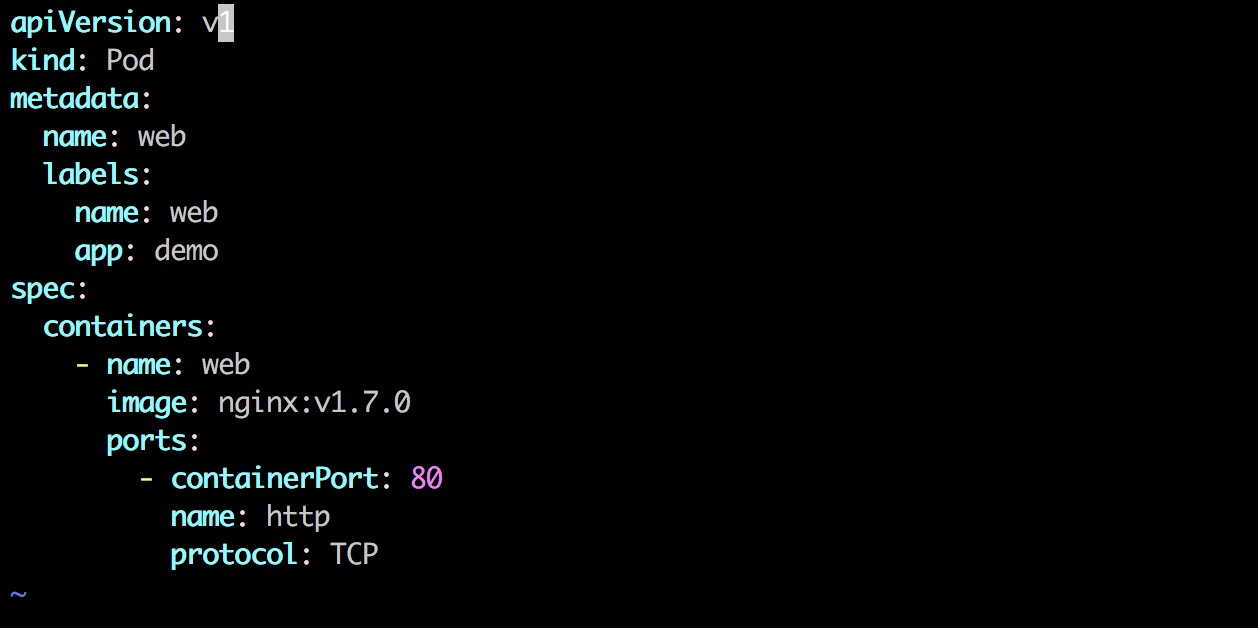
\includegraphics[width=\textwidth,scale=0.6]{../kubernetes-101/images/kubernetes-pod.png}
	\begin{itemize}
			\item pod是kubernetes里的最小单元,相当于一个VM,
			\item 一个pod里可以运行多个容器,他们共享主机名,IP,PORT, 存储
			\item 如果需要对pod做水平扩展,便可以使用replication controllers,
	\end{itemize}
	
	
}

\section{service}

\frame{
	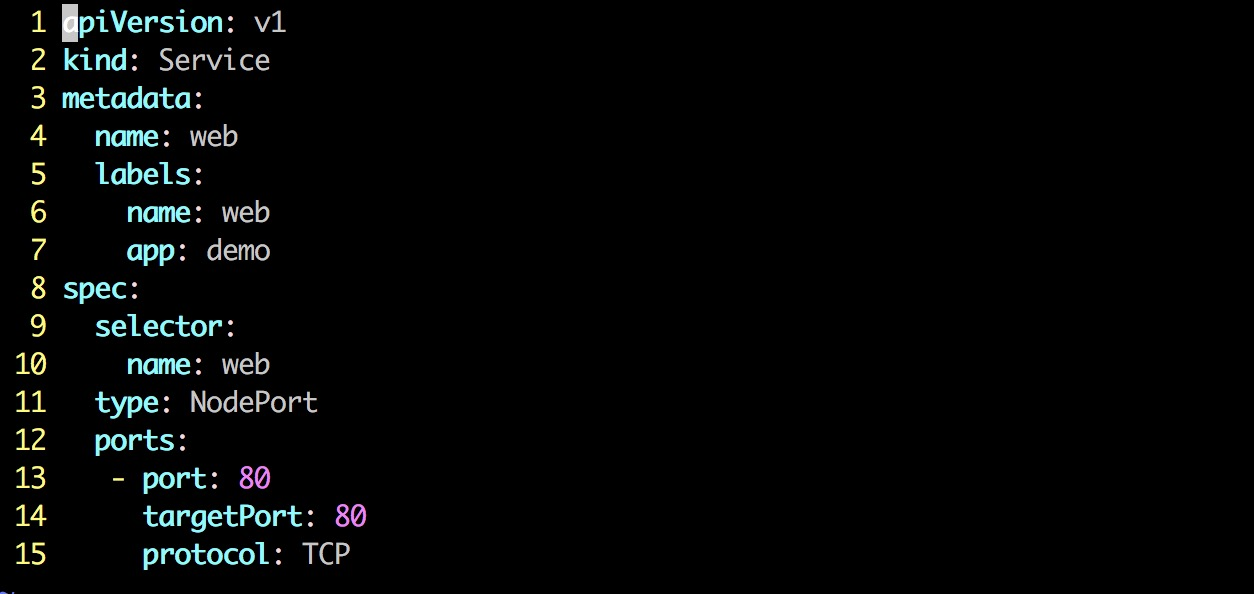
\includegraphics[width=\textwidth,scale=0.6]{../kubernetes-101/images/kubernetes-svc.png}

	\begin{itemize}
			\item 提供对外访问
			\item 支持 nodePort, loadBlance
	\end{itemize}
}
\end{document}
